%\setchapterimage{Fond_CIN.png}
\setchapterpreamble[u]{\margintoc}

\chapter{Génie électrique en tension alternative}


%\marginnote[4cm]{
%\UPSTIcompetence[2]{B2-10}
%}

%\marginnote[6cm]{\textbf{Emilien Durif}, \textit{Approche énergétique}, Lycée La Martinière Monplaisir, Lyon.}

\section{Signaux périodiques}

\subsection{Caractéristique des signaux périodiques}

\begin{marginfigure}
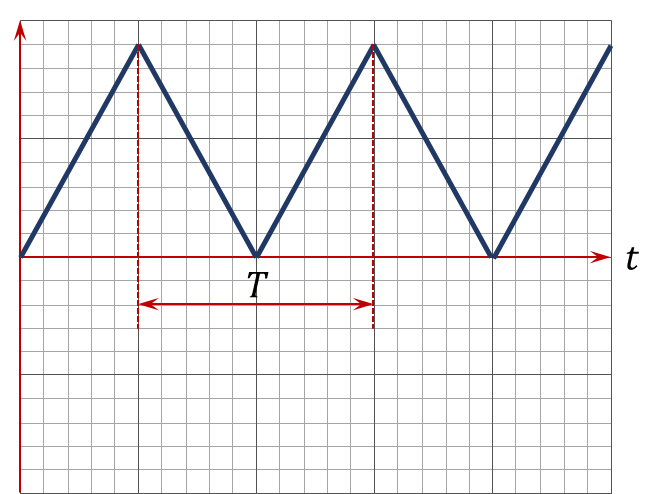
\includegraphics[width=\linewidth]{fig_01}
\caption{Signal périodique \label{fig:ge:cours:01}}
\end{marginfigure}

\begin{defi}[Signal périodique]
Un signal $s(t)$ est dit périodique de période $T$ si $\forall t$, $s(t)=s(t+T)$.
\end{defi}

\begin{defi}[Caractéristiques]
On peut définir : 
\begin{itemize}
\item la fréquence du signal, en Hertz \si{Hz}, $f=\dfrac{1}{T}$;
\item la pulsation, pour un régime sinusoïdal, en \si{rad.s^{-1}} :  $\omega = 2\pi f$;
\item la valeur maximale (ou de crête). 
\end{itemize}
\end{defi}

\subsection{Valeur moyenne}
\begin{marginfigure}
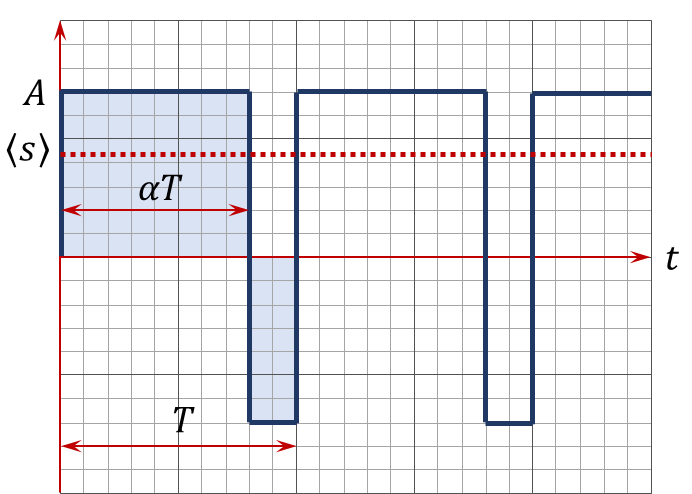
\includegraphics[width=\linewidth]{fig_02}
\caption{Valeur moyenne\label{fig:ge:cours:02}}
\end{marginfigure}


\begin{marginfigure}
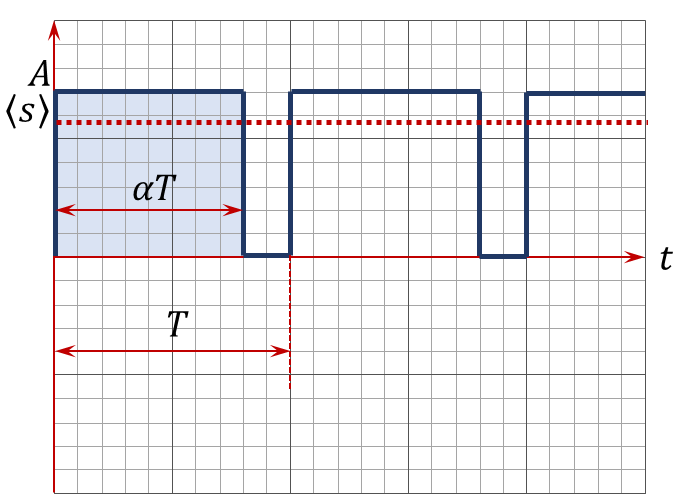
\includegraphics[width=\linewidth]{fig_03}
\caption{Valeur moyenne\label{fig:ge:cours:03}}
\end{marginfigure}

\begin{defi}[Valeur moyenne]
Valeur de la grandeur continue qui créerait la même aire qu'un signal périodique sur une période $T$.
On a alors : 
$$\langle s \rangle = \dfrac{1}{T} \int\limits_{t_0}^{t_0+T} s(t)\; \dd t.$$
\end{defi}

\begin{prop}
Si $s(t) = s_1(t)+s_2(t)$ alors  $\langle s \rangle = \langle s_1 \rangle+\langle s_2 \rangle$.
\end{prop}

La valeur moyenne est celle mesurée par un multimètre en position \textbf{DC} ou \textbf{=}.

Le courant moyen d'un courant périodique serait équivalant au courant continu qui tranporterait la même quantité d'électricité que celle tranportée durant une période.

\subsection{Valeur efficace}
\begin{defi}[Valeur efficace]
La valeur efficace $S$ ou $\indice{S}{eff}$ du signal $s(t)$ est donnée par  
$$\indice{S}{eff} = \sqrt{\dfrac{1}{T} \int\limits_{t_0}^{t_0+T} s^2(t)\; \dd t} = \sqrt{\langle s^2 \rangle}.$$

En anglais on parle de Root Mean Square (RMS).
\end{defi}


La valeur moyenne est celle mesurée par un multimètre en position $\sim$ 
ou \textbf{AC+DC} ou \textbf{RMS}.

Le courant efficace d'un courant périodique serait équivalant au courant continu qui produirait le même dégagement de chaleur que lui dans une résistance durant une période.

Pour la figure \ref{fig:ge:cours:02} la valeur moyenne du signal est de 4,2.
$\indice{S}{eff} = \sqrt{\dfrac{1}{T} \int\limits_{t_0}^{t_0+T} s^2(t)\; \dd t}$
$=\sqrt{\dfrac{1}{10} \left( \int\limits_{0}^{8} 7^2(t)\; \dd t + \int\limits_{8}^{10} 7^2(t)\; \dd t\right)}$
$=\sqrt{\dfrac{1}{10} \left( \int\limits_{0}^{8} 7^2(t)\; \dd t + \int\limits_{8}^{10} 7^2(t)\; \dd t\right)}.$
$=\sqrt{\dfrac{1}{10} \left( 49 \times 8 + 49 \times 2\right)}=7$



Pour la figure \ref{fig:ge:cours:03} la valeur moyenne du signal est de 5,6. Dans ce cas, la valeur efficace est de $\indice{S}{eff} = 6,26$.

\subsection{Décompostion d'un signal périodique}
\begin{prop}
Un signal périodique $s(t)$ est déocomposable en une somme d'un signal alternarif $s_a(t)$ et d'un signal constant : 
$$ s(t)= \langle s \rangle + s_a(t) .$$

On appelle  $\langle s \rangle$ composante continue et $s_a(t)$ composante alternative ou d'ondulation. Par ailleurs, on a alors $\langle s_a \rangle = 0$. 
\end{prop}

\begin{figure}[!h]
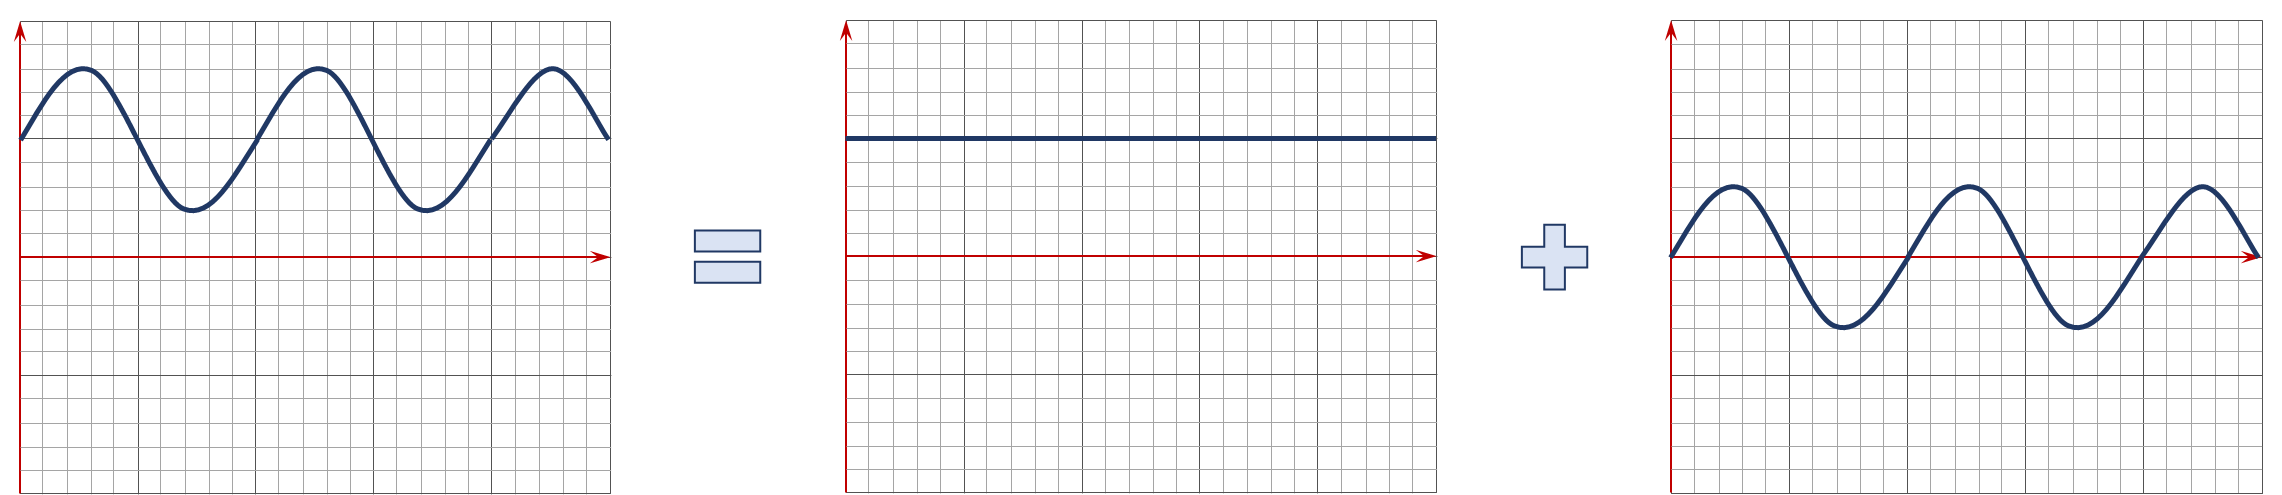
\includegraphics[width=\linewidth]{fig_04}
\caption{Décomposition d'un signal périodique\label{fig:ge:cours:04}}
\end{figure}

Sur les oscilloscopes : 
\begin{itemize}
\item en couplage DC le signal complet $s(t)$ est affiché;
\item en couplage AC seule la composante alternative $s_a(t)$ est affichée.
\end{itemize}

On a $\indice{S}{eff}^2 = \langle s \rangle^2 + \indice{S_a}{eff}^2$.

\subsection{Signal alternatif et sinusoïdal}

\begin{marginfigure}
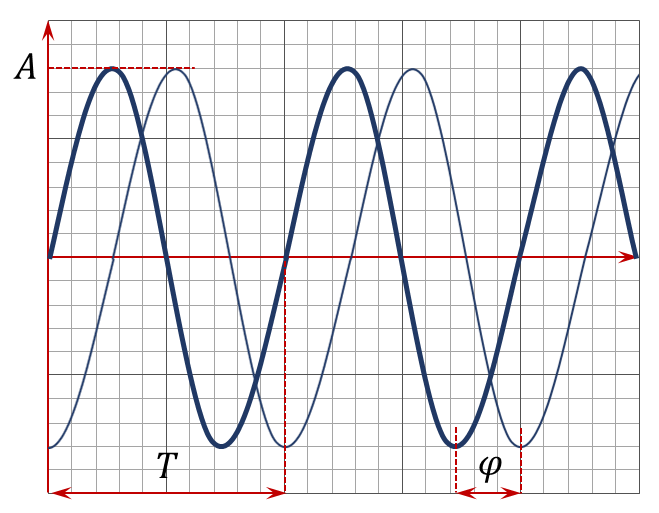
\includegraphics[width=\linewidth]{fig_05}
\caption{Signal alternatif sinusoïdal \label{fig:ge:cours:05}}
\end{marginfigure}
\begin{defi}
On note $s(t)=A\sin\left(\omega t + \varphi\right)$ avec : 
\begin{itemize}
\item  $A$ amplitude du signal;
\item  $\omega$ pulsation en $\si{rad.s^{-1}}$ tel que $\omega = 2\pi f = \dfrac{2\pi}{T}$;
\item  $\varphi$  phase à l'instant $t$.
\end{itemize}
\end{defi}


\begin{resultat}
Pour un signal sinusoïdal, on a (voir paragraphe \ref{calcul:01}) $\indice{S}{eff}= \dfrac{A}{\sqrt{2}}$.
\end{resultat}



\subsection{Puissance électrique}

\begin{defi}[Puissance instantanée]
Soit un dipôle parcouru par un courant $i(t)$ et soumis à une tension $u(t)$.
La puissance instantanée s'exprime par 
$$p(t)=u(t) i(t).$$

\end{defi}

\begin{resultat}
Si $u(t)=U\cos\left(\omega t + \varphi\right)$
et 
$i(t)=I\cos\left(\omega t + \varphi'\right)$ 
alors on montre que 

$p(t)=\dfrac{UI}{2}\left( \cos\left(2\omega t + \varphi + \varphi' \right)+\cos\left(\varphi -\varphi' \right)\right)$
\end{resultat}

\begin{defi}[Puissance active]
Soit un dipôle parcouru par un courant $i(t)$ et soumis à une tension $u(t)$.
La puissance active $P$ en \si{W} s'exprime par :
$$P = \langle p(t) \rangle = \langle u(t) i(t) \rangle  =\dfrac{1}{T} \int\limits_{0}^{T} u(t) i(t)\; \dd t. $$
\end{defi}


\subsubsection{Puissance reçue par une résistance}
\begin{marginfigure}
\centering
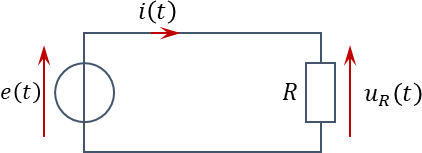
\includegraphics[width=\linewidth]{sch_01}
\caption{Circuit R \label{fig:ge:cours:sch_01}}
\end{marginfigure}

La source de tension $e$ est de la forme $e(t)=E\cos\left(\omega t + \varphi\right)$. En écrivant la loi des mailles dans le ciruit de la figure \ref{fig:ge:cours:sch_01} on a $u_R(t)=e(t)$. Par ailleurs, $u_R(t) = R i(t)$; donc $i(t)=\dfrac{E}{R}\cos \left(\omega t + \varphi\right)$.
$u_R(t)$ et $i(t)$ sont donc en phase. 

La puissance instantanée reçue par le dipôle est $p(t) =\dfrac{E^2}{R}\cos^2 \left(\omega t + \varphi\right) $.

La puissance active est $P = \dfrac{E^2}{2R}$
% =  \dfrac{\left(\indice{E}{eff}\sqrt{2}\right)^2}{2R}
$=  \dfrac{\indice{E}{eff}^2}{R}$.
Par ailleurs, $I = \dfrac{E}{R} \Rightarrow \indice{I}{eff}\sqrt{2} = \dfrac{\indice{E}{eff}\sqrt{2}}{R} $ et $\indice{I}{eff} = \dfrac{\indice{E}{eff}}{R}$; donc $P=  R\indice{I}{eff}^2$.

\subsubsection{Puissance reçue par un condensateur}
\begin{marginfigure}
\centering
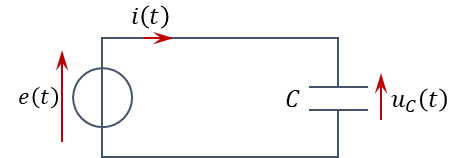
\includegraphics[width=\linewidth]{sch_02}
\caption{Circuit RC \label{fig:ge:cours:sch_02}}
\end{marginfigure}

La source de tension $e$ est de la forme $e(t)=E\cos\left(\omega t + \varphi\right)$. En écrivant la loi des mailles dans le ciruit de la figure \ref{fig:ge:cours:sch_02} on a $u_C(t)=e(t)$. Par ailleurs,  $i(t)=C\deriv{u_c(t)}{}$.

On a donc, $i(t)=-CE\omega\sin\left(\omega t + \varphi\right)$.

Or, $-\sin(x) =\cos(x+\dfrac{\pi}{2})$. On a donc 
$i(t)=CE\omega\cos\left(\omega t + \varphi+\dfrac{\pi}{2}\right)$. La tension est donc << en retard >> sur le courant. 


La puissance instantanée s'exprime donc par $p(t)=i(t) u_c(t)$
$= -CE\omega^2\cos\left(\omega t + \varphi\right)\sin\left(\omega t + \varphi\right)$.

La puissance active se calcule donc ainsi :
$P= -\dfrac{CE\omega^2}{T}\underbrace{\int\limits_{0}^{T} \cos\left(\omega t + \varphi\right)\sin\left(\omega t + \varphi\right)\; \dd t}_{0}=0$.
%
%En passant en notation complexe, on a $\underline{i}(t)=C\deriv{\underline{u_c}(t)}{}$
%$=jC\omega\underline{u_c}(t)$ et $e(t)=Ee^{j\left(\omega t + \varphi\right)}$. On a donc 
%$\underline{i}(t)=jC\omega Ee^{j\left(\omega t + \varphi\right)}$
%$ = jC\omega E \left(\cos\left(\omega t + \varphi\right)+j\sin\left(\omega t + \varphi\right)\right)$
%$ = C\omega E \left(j\cos\left(\omega t + \varphi\right)-\sin\left(\omega t + \varphi\right)\right)$
%.
%
%On a alors, $i(t) =Re\left(\underline{i}(t)\right) $ $=-C\omega E \sin\left(\omega t + \varphi\right)$



\section{Alimentation monphasée}

\begin{marginfigure}
\centering
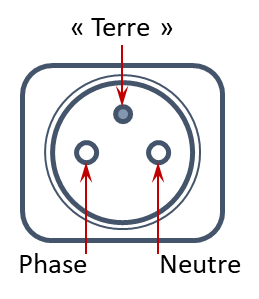
\includegraphics[width=.6\linewidth]{fig_06}
\caption{Prise électrique \label{fig:ge:cours:06}}
\end{marginfigure}

Aux bornes d'une prise électrique domestique, l'alimentation est sinusoïdale monophasée. Entre la phase et le neutre on mesure une tension simple $v(t)$ dont la valeur efficace est de $\SI{230}{V}$.

Ainsi l'amplitude du signal est de \SI{325}{V}.

\begin{marginfigure}
\centering
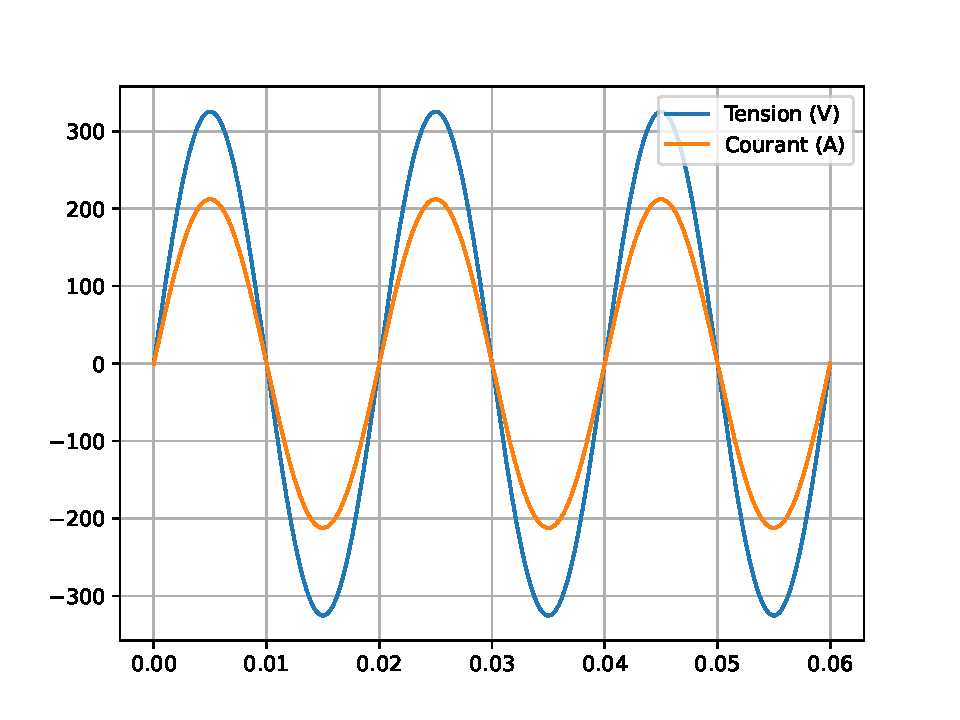
\includegraphics[width=\linewidth]{plt_01.pdf}
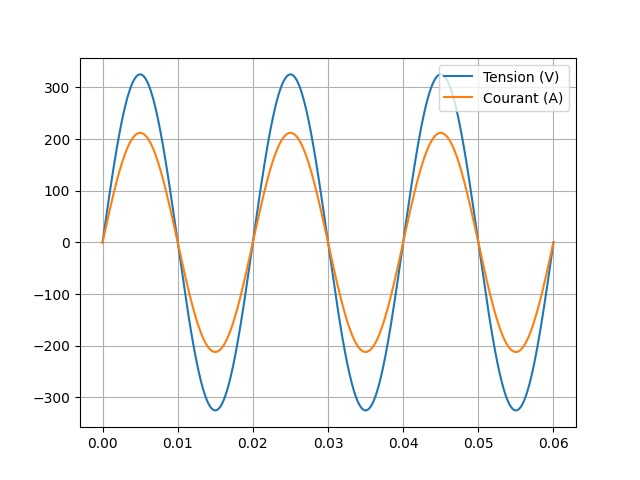
\includegraphics[width=\linewidth]{plt_01.png}
\caption{ Tension et courant sinusoïdaux\label{fig:ge:cours:plt:01}}

\end{marginfigure}

La tension et le courant distribués sont sinusoïdaux. 


\section{Quelques calculs}

\subsection{Intégrale $\dfrac{1}{T} \int\limits_{0}^{T} A^2 \sin^2(\omega t + \varphi)\; \dd t.$ \label{calcul:01}}

$I = \dfrac{1}{T} \int\limits_{0}^{T} A^2 \sin^2(\omega t + \varphi)\; \dd t.$
$= \dfrac{ A^2}{2 T} \int\limits_{0}^{T} \left( 1 - \cos\left( 2\left(\omega t + \varphi\right)\right)\right)\; \dd t$


$= {\dfrac{ A^2}{2 T}\left( \left[t\right]_{0}^{T} -  \left[\dfrac{1}{2\omega}\sin\left( 2\left(\omega t + \varphi\right)\right)\right]_{0}^{T}  \right)}$

$= {\dfrac{ A^2}{2 T}\left( T -  \dfrac{1}{2\omega}\left[
\sin\left( 2\left(\omega T + \varphi\right)\right)
- \sin\left( 2\left(\omega \times 0 + \varphi\right)\right)\right]  \right)}$

$= {\dfrac{ A^2}{2 T}\left( T -  \dfrac{1}{2\omega}\left[
\sin\left( 2\left(\omega T + \varphi\right)\right)
- \sin\left( 2 \varphi\right)\right]  \right)}$. 

$= {\dfrac{ A^2}{2 T}\left( T -  \dfrac{1}{2\omega}\left(
\sin\left( 2\omega T \right)\cos\left( 2\varphi\right)
+\cos\left( 2\omega T \right)\sin\left( 2\varphi\right)
- \sin\left( 2 \varphi\right)\right)  \right)}$. 

On a $\omega = \dfrac{2\pi}{T}$.

$I= {\dfrac{ A^2}{2 T}\left( T -  \dfrac{1}{2\dfrac{2\pi}{T}}\left(
\sin\left( 2\dfrac{2\pi}{T} T \right)\cos\left( 2\varphi\right)
+\cos\left( 2\dfrac{2\pi}{T} T \right)\sin\left( 2\varphi\right)
- \sin\left( 2 \varphi\right)\right)  \right)}$ 

$ = \dfrac{ A^2}{2 T}\left( T -  \dfrac{T}{4\pi}\left(
\sin\left( 2\varphi\right) - \sin\left( 2 \varphi\right)\right)  \right) $
$ =\dfrac{A^2}{2}$





%\subsection{Valeur efficace d'un signal sinusoïdal $\indice{S}{eff} = \sqrt{\dfrac{1}{T} \int\limits_{0}^{T} A^2 \sin^2(\omega t + \varphi)\; \dd t}.$}
%
%Pour un signal périodique, calculons la valeur efficace : 
%$\indice{S}{eff} = \sqrt{\dfrac{1}{T} \int\limits_{0}^{T} A^2 \sin^2(\omega t + \varphi)\; \dd t}.$
%$= \sqrt{\dfrac{ A^2}{2 T} \int\limits_{0}^{T} \left( 1 - \cos\left( 2\left(\omega t + \varphi\right)\right)\right)\; \dd t}$
%$= \sqrt{\dfrac{ A^2}{2 T}\left( \left[t\right]_{0}^{T} -  \left[\dfrac{1}{2\omega}\sin\left( 2\left(\omega t + \varphi\right)\right)\right]_{0}^{T}  \right)}$
%
%$= \sqrt{\dfrac{ A^2}{2 T}\left( T -  \dfrac{1}{2\omega}\left[
%\sin\left( 2\left(\omega T + \varphi\right)\right)
%- \sin\left( 2\left(\omega \times 0 + \varphi\right)\right)\right]  \right)}$
%
%$= \sqrt{\dfrac{ A^2}{2 T}\left( T -  \dfrac{1}{2\omega}\left[
%\sin\left( 2\left(\omega T + \varphi\right)\right)
%- \sin\left( 2 \varphi\right)\right]  \right)}$. 
%
%
%Avec $\varphi=0$, 
%$\indice{S}{eff}= \sqrt{\dfrac{ A^2}{2 T}\left( T -  \dfrac{\sin\left( 2\omega T \right)}{2\omega}
%  \right)}$
%  $= \sqrt{\dfrac{ A^2}{2 T}\left( T -  \dfrac{\sin\left( 2\dfrac{2\pi}{T} T \right)}{2\dfrac{2\pi}{T}}  \right)}$
%  $= \sqrt{\dfrac{ A^2}{2 T}T }$ $= \dfrac{A}{\sqrt{2}}$.

\subsection{Notation complexe}
\marginnote{Rappel : 
\begin{itemize}
\item forme algébrique : $\underline{z} = a+j b$;
\item forme trigonométrique $\underline{z} = Z\left(\cos \varphi + j \sin \varphi \right)$;
\item forme exponentielle $\underline{z} = Z e^{j \varphi}$.
\end{itemize}}

\begin{defi}
Soit un signal mathématique $x(t)=X \cos\left( \omega t + \varphi \right)$. On lui associe 
une grandeur complexe: $\underline{x}(t)=X e^{j\left(\omega t + \varphi\right)}$.
\end{defi}

\begin{resultat}[Retour au signal réel]
\begin{itemize}
\item $x(t) = Re\left(\underline{x}(t)\right)$
\item $\varphi ... $
\end{itemize}
\end{resultat}